\documentclass[a4,12pt,graphicx,caption,rotating]{article}

\usepackage[utf8]{inputenc}
\usepackage[spanish]{babel}
\usepackage[margin=1.5cm]{geometry}
\usepackage{graphicx}
\usepackage{hyperref}

\begin{document}
\begin{titlepage}
 
\begin{center}
 
{\Large TECNOLOGÍAS ESPECÍFICAS DE LA INGENIERÍA INFORMÁTICA}\\
 
{\Large Grado en Ingeniería en Informática}\\[2cm]
 
{\Large Curso 2013-2014}\\[3cm]
 
{\Huge Trabajo parte DIS}\\
 
{\Huge Introducción a Octave utilizando \LaTeX y Git}\\[4cm]
 
{\Large Alumno: José Joaquín Pastor Martínez}\\[3cm]
 
{\Large UNIVERSIDAD DE MURCIA}
 
\end{center}
 
\end{titlepage}
 
\tableofcontents
\newpage

\section{Introducción}
GNU Octave es un lenguaje de alto nivel destinado para el cálculo numérico, sólo opera con números. Provee una interfaz sencilla, orientada a la línea de comandos (consola), que permite la resolución de problemas numéricos, lineales y no lineales, además permite la ejecución de scripts y puede ser usado como lenguaje orientado al procesamiento por lotes.

Octave nació alrededor del año 1988, y fue concebido originalmente para ser usado en un curso de diseño de reactores químicos. El desarrollo real de comenzó en 1992. La primera alfa fué publicada en 1993, y en 1997 se publicó la versión 1.0.
\cite{iniOctave}
\section{Iniciar y salir de Octave}
Para iniciar octave hay que ejecutar la instrucción \emph{octave} en una consola. Aparecerá la siguiente ventana:
\begin{verbatim}
GNU Octave, version 3.6.2
Copyright (C) 2012 John W. Eaton and others.
This is free software; see the source code for copying conditions.
There is ABSOLUTELY NO WARRANTY; not even for MERCHANTABILITY or
FITNESS FOR A PARTICULAR PURPOSE.  For details, type `warranty'.

Octave was configured for "x86_64-pc-linux-gnu".

Additional information about Octave is available at http://www.octave.org.

Please contribute if you find this software useful.
For more information, visit http://www.octave.org/help-wanted.html

Read http://www.octave.org/bugs.html to learn how to submit bug reports.

For information about changes from previous versions, type `news'.

octave:1>
\end{verbatim}

Para salir de octave usaremos el comando \emph{quit} o \emph{exit}.

\subsection{Instrucciones de utilidad}
\begin{itemize}
\item$>$pwd: para mostrar el directorio en el que nos encontramos.
\item$>$ls: para mostrar una lista de los ficheros y los directorios del directorio actual.
\item$>$cd ruta: para cambiar de directorio.
\item$>>$cd ..: para ir al directorio padre.
\item$>$diary: volcar lo mostrado en el transcurso de la ejecución del programa al fichero ‘diary’ de la carpeta por defecto.
\item$>>$diary fichero: el fichero ‘diary’ se guardará en el fichero indicado.
\item$>>$diary off: para el guardado.
\item$>$help comando: muestra la ayuda sobre el comando indicado.
\item$>$history: muestra una lista con los comandos ejecutados.
\item$>$save archivo: guardar la sesión en un archivo.
\item$>$load archivo: cargar la sesión del archivo.
\end{itemize}
Los comandos pueden recuperarse con la \emph{flecha hacia arriba}, o escribiendo el inicio del comando y pulsar la \emph{flecha hacia arriba}, y navegar por los comandos ejecutados.
\subsection{Operaciones básicas}
\begin{itemize}
\item= \emph{asignacion}
\item+ \emph{suma}
\item- \emph{resta}
\item* \emph{multiplicación}
\item.* \emph{multiplicación de matrices elemento por elemento (deben coincidir el número de columnas con el número de filas)}
\item/ \emph{división derecha}
\item exp \emph{exponencial}
\item log \emph{logaritmo neperiano}
\item log10 \emph{logaritmo base 10}
\item sin \emph{seno}
\item cos \emph{coseno}
\item abs \emph{valor absoluto}
\item sqrt \emph{raíz cuadrada}
\item round \emph{redondeo al entero más cercano}
\item floor \emph{redondea por defecto}
\item ceil \emph{redondea por exceso}
\item ' \emph{transpuesta}
\end{itemize}
\section{Variables}
Podemos asignar variables con determinados nombres a las expresiones numéricas (números, constantes). Los nombres son sensibles a mayúsulas y minúsculas, el máximo de caracteres que deben tener es de 31 caracteres, deben empezar or una letra y pueden contener letras, números y el símbolo '\_'. Las variables se crean escribiendo el nombre que le queramos dar y asignándole el valor con el operador de asignación. El acceso a la variable se realiza escribiendo el nombre asignado.
\begin{verbatim}
>a=1/3
\end{verbatim}
Cuando se asigna otro valor se machaca en anterior
\begin{verbatim}
>a=1/3
>a=1/6
>a
a=0.16667
\end{verbatim}
Las variables creadas se guardan en una lista de variables.
\begin{itemize}
\item>whos: obtener la lista de vaiables guardadas.
\end{itemize}
Las variables guardadas pueden ser borradas.
\begin{itemize}
\item$>$clear: borra todas las varianles
\item$>>$clear a: borra la variable indiaca (en este caso a).
\end{itemize}
Pueden colocarse varios comandos en una misma línea separándolos con ',', si no se quiere que se muestre el resultado de algún comando se finaliza el comando con ';'.

Se permiten comentarios, de gran ayuda a la hora de realizar scripts para ejecutar.
\begin{itemize}
\item\% línea de comentario, todo lo que esté a su derecha se considera comentario.
\end{itemize}
Se puede extender un comando a más de una línea con '...'.
\begin{verbatim}
>esto\_es\_muy\_largo...
>=17
esto\_es\_muy\_largo = 17
\end{verbatim}
\subsection{Variables predefinidas}
\begin{itemize}
\item ans último resultado
\item pi = 3.1416
\item e = 2.7183
\item i, j número imaginario
\item Inf infinito
\item NaN indeterminado
\end{itemize}
\section{Vectores}
Un vector es definido como un conjunto de datos a los cuales se accede por medio de índices. Es una matriz de una dimensión.

La forma en la que octave se definen vectores es utilizando corchete []. Los elementos de una fila se separan con un espacio ' ' o una coma ','.
\begin{verbatim}
> v= [1,2,3,5,7,11]
v =

    1    2    3    5    7   11
\end{verbatim}
Las columnas por su parte se separan mediante puntos y comas ';'.
\begin{verbatim}
> w= [1;2;3;5;7;11]
w =

    1
    2
    3
    5
    7
   11
\end{verbatim}
\subsection{Secuencias}
En octave podemos crear vectores de secuencas utilizando los dos puntos, p:q:r, donde p sería el valor en el que se iniciaría la secuencia, \emph{r} el valor final y \emph{q} el intervalo. El valor \emph{q} es opcional y si se obvía el intervalo por defecto es 1.
\begin{verbatim}
> 1:10
ans =

    1    2    3    4    5    6    7    8    9   10
> 1:2:10
ans =

    1    3    5    7    9
\end{verbatim}
Además hay otras dos funciones para crear vectores con secuencias separadas x valores, \emph{linspace} y \emph{logspace}. El primero separa los números uniformemente y el segundo logarítmicamente.
\begin{verbatim}
> linspace(0,15,6)
ans =

    0    3    6    9   12   15
\end{verbatim}
Hay dos funciones especiales para crear filas o columnas de unos o ceros, \emph{ones} y \emph{zeros}
\begin{verbatim}
> ones(1,5)
ans =

   1   1   1   1   1
\end{verbatim}
\subsection{Funciones sobre vectores}
\begin{itemize}
\item length \emph{devuelve la longitud del vector}
\end{itemize}
\section{Matrices}
Las matrices se introducen por filas, cuyos elementos se separan con ' ' o ',', y que se separan unas de otras con ';'.
\begin{verbatim}> M=[1 2 3; 6 2 0; 0 1 -2]
M =

   1   2   3
   6   2   0
   0   1  -2
\end{verbatim}
La transpuesta de esta matriz se realizaría fácilmente con el simbolo de trasposición M'.
\begin{verbatim}
> M'
ans =

   1   6   0
   2   2   1
   3   0  -2
\end{verbatim}
Se pueden realizar operaciones entre matrices como su suma de matrices \emph{(M+N)}, resta de matrices \emph{(M-N)}, multiplicación de matrices \emph{(M*N)\footnote{M debe tener el mismo número de colúmnas que N.}}, multiplicación elemento a elemento \emph{(M.*N)\footnote{Aunque no tiene mucho sentido a la hora de trabajar con matrices en el cálculo numérico si que puede ser útil si se consideran las matrices con datos ordenados en forma matricial.}}, calcular su matriz inversa \emph{inv(M)}, potenciación o divisiones izquierda y derecha.

A los elementos de vectores y matrices se puede acceder por índice, esto es por su posición en el mismo. El índice empieza por 1, siendo V(1) el primer elemento en el caso de los vectores y M(1,1) el primero en el caso de las matrices. Se puede obtener una partde de un vector indicando los índices con V(2:5). Así como también se puede obetener una fila de una matriz sin seleccionar la columna del elemento del indice y poniéndola con ':', por ejemplo: M(2,:) nos devolvería el vector de la fila 2.
\subsection{Resolución de ecuaciones}
En octave se pueden resolver sistemas de ecuaciones de una forma sencilla utilizando matrices.

Partiendo de las dos ecuaciones:
\begin{displaymath}
ax+by=c
\end{displaymath} 
\begin{displaymath} 
dx+ey=f
\end{displaymath} 
Construimos las matrices siguiente:
\begin{verbatim}
> a=[a b;d e]
a =

   a   b
   d   e

> b=[f;c]
b =

   c
   f
\end{verbatim}
Donde en la primera matriz colocamos los coeficientes que acompañan a las incógnitas, si en una encuación no aparece una incognita pondremos un 0 en su posición en la matriz. Y en la segunda pondremos los valores de la parte derecha de las ecuaciones. Finalmente el sistema se resolvería:
\begin{verbatim}
> res=a\b
res =

   X
   Y
\end{verbatim}
\section{Scripts en octave}
Para explicar esta parte voy a suponer que se tienen unos conocimientos básicos de programación, ya que no es este documento el lugar donde explicar IFs, bucles, funciones, etc... por lo que únicamente mostraré la forma de utlizarlos en octave.

Los scripts en Octave son archivos con extensión \emph{.m}. Octave es un programa para el cálculo numérico, por lo que las posibilidades de los scripts son limitadas. Aún así el programa nos da la posibilidad de utilizar operadores lógicos, condiciones, funciones y bucles.
\subsection{Operadores lógicos}
Los operadores lógicos permitidos son:
\begin{center}
\&, |, \~~
\end{center} 
que corresponden a and, or y negación respectivamente.
\subsection{Condiciones}
\subsubsection{IF}
\begin{verbatim}
            IF condición1
                cuerpo1
            ELSEIF condición2
                cuerpo2
            ELSE
                cuerpo3
            ENDIF
\end{verbatim} 
\subsubsection{SWITCH}
\begin{verbatim}
            SWITCH expresión
            CASE etiqueta1
                listadecomandos1
            CASE etiqueta2
                listadecomandos2
             ... 
            OTHERWISE
                listadecomandosFinal
            ENDSWITCH 
\end{verbatim}
\subsection{Bucles}
\subsubsection{FOR}
\begin{verbatim}
            FOR var = expresión
                cuerpo
            ENDFOR
\end{verbatim}
\subsubsection{DO-UNITL}
\begin{verbatim}
            DO
                cuerpo
            UNTIL (condición)
\end{verbatim}
\subsubsection{WHILE}
\begin{verbatim}
            WHILE (condicion)
                cuerpo
            ENDWHILE
\end{verbatim}
\subsection{Funciones}
\begin{verbatim}
            FUNCTION [salida1, salida2] = nombre_funcion (argumentos)
              cuerpo
            ENDFUNCTION
\end{verbatim}

Estas funciones además de en un script se pueden definir en una consola ejecutando octave y utilizarlas posteriormente utilizando su nombre como si de una función predefinida por octave se tratase.
\subsection{Recoger información del usuario}
Si queremos que el usuario aporte alguna información para el cálculo debemos ejecutar el comando \emph(input).
\begin{verbatim}
            kilometros = input('Introduzca los kilometros recorridos: ');
\end{verbatim}
\subsection{Ejecución}
Para ejecutar un programa en octave debemos arrancar el programa en una consola y escribir el nombre del script en la consola de octave.

\section{Grafos en octave}
Para la asignatura de Sistemas Inteligentes hemos realizado una práctica para planificar y programar el trabajo de un taladro perforador automático para que realice su trabajo en un tiempo mínimo y así, poder realizar el mayor número de placas perforadas en un tiempo dado.
En el algoritmo genético que utilizamos para resolver el problema debemos modificar las variables del tamaño de la población y del número de generaciones para ver como interceden en la mejora de la solución obtenida, pero aumentar el valor de estas variables conlleva un aumento del tiempo de ejecución del algoritmo.
Los datos del tiempo de ejecución del caso del tamaño de la población están en popsize.txt.\cite{uno}
Y la gráfica tamaño tiempo la obtenemos en octave ejecutando:
\begin{verbatim}
            popsize = load("popsize.txt");
            plot (popsize (:,1), popsize (:,2));
\end{verbatim}
La gráfica resultante se puede ver en la figura 1.
\begin{figure}[t]
\begin{center}
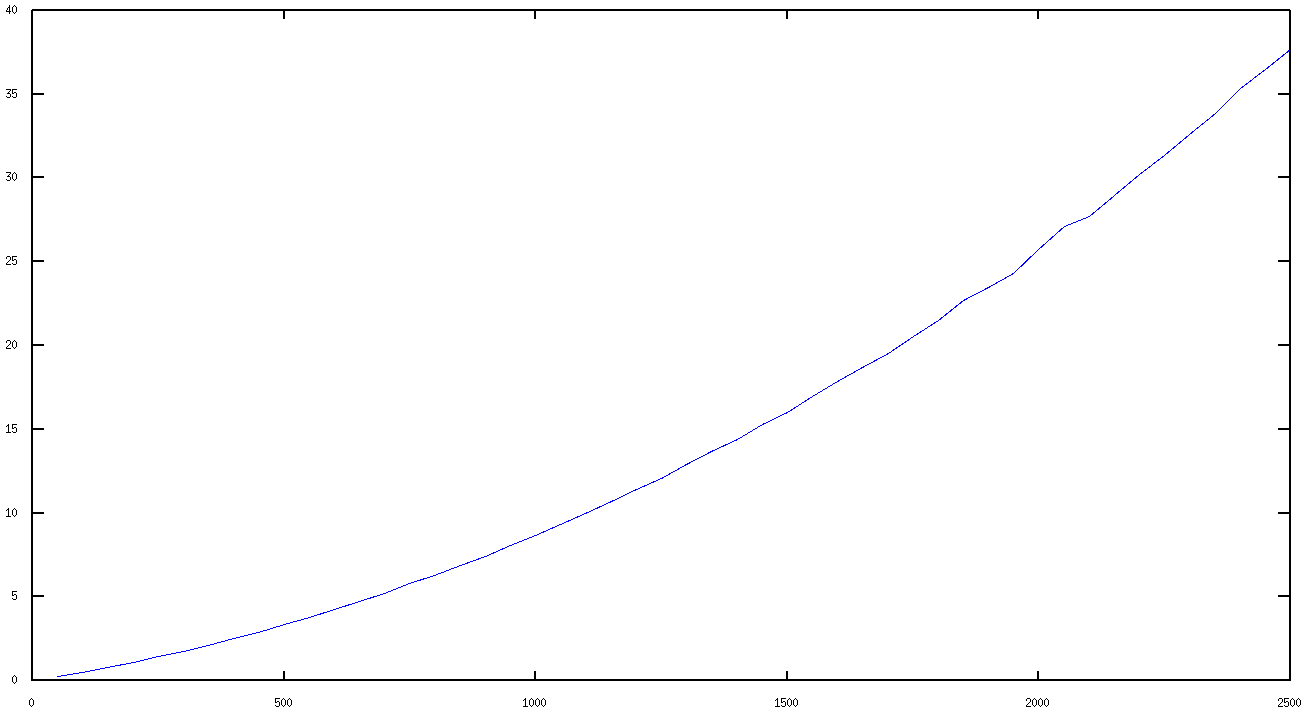
\includegraphics[width=0.9\textwidth]{graph/popsize}
\end{center}
\caption{Grafo del tiempo de ejecución según el tamaño de población}
\label{fig:popsize}
\end{figure}

Los datos del tiempo de ejecución del caso del número de generaciones están en ngen.txt.
Y la gráfica número de generaciones tiempo la obtenemos en octave ejecutando:
\begin{verbatim}
            ngen = load("ngen.txt");
            plot (ngen (:,1), ngen (:,2));
\end{verbatim}
\begin{figure}[t]
\begin{center}
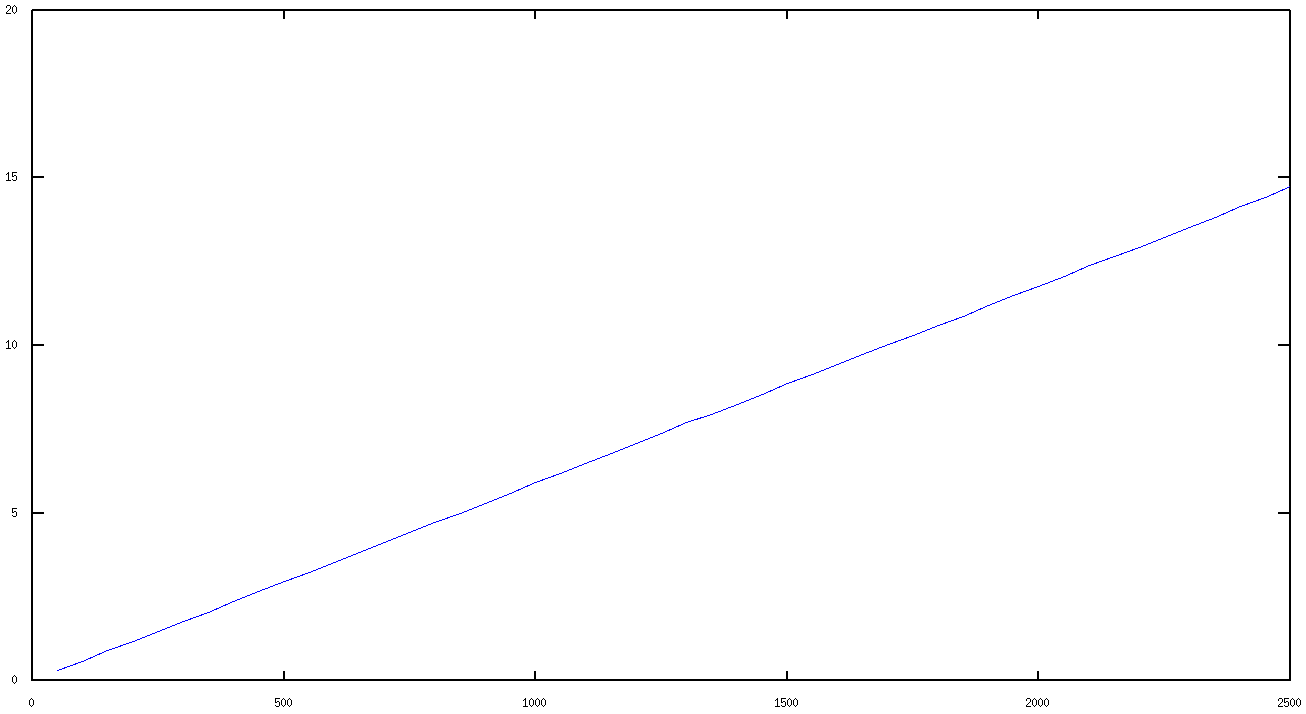
\includegraphics[width=0.9\textwidth]{graph/ngen}
\end{center}
\caption{Grafo del tiempo de ejecución según el número de generaciones}
\label{fig:ngen}
\end{figure}
La gráfica resultante se puede ver en la figura 2.
\begin{thebibliography}{X}
	\bibitem{1} \textsc{Jose Maria Valiente Cifuentes},
		\textit{Manual de iniciación a GNU Octave}
		\url{http://softlibre.unizar.es/manuales/aplicaciones/octave/manual_octave.pdf}
	\bibitem{2} \textsc{Barry O'Donovan},
		\textit{GNU Octave - An Introduction}
		\url{http://linuxgazette.net/109/odonovan.html}
	\bibitem{3}
		\textit{Octave Programming Tutorial/Vectors and matrices}
		\url{http://en.wikibooks.org/wiki/Octave_Programming_Tutorial/Vectors_and_matrices}
	\bibitem{4}
		\textit{Octave-Forge}
		\url{http://octave.sourceforge.net/}

}
\end{thebibliography}
\end{document}
